This section will explain the basic theory and concept behind Ambient Occlusion. Besides covering the basic concept and math behind ambient occlusion it will also be covered how texture lookup into light probe images are performed. The chapter will conclude with a discussion of the disadvantages of ambient occlusion.
\section{The Basic Concept}
Ambient Occlusion works by seeing how much of an external envirornment can be seen from each surface point on the object or scene to be rendered. The more of the external envirornment that can be seen, the more ambient lighting that point will recieve. This type of illumination is therefore often called "sky light" in production, because it simulates how a model would be lighted on an overcast day, since the light from ambient occlusion is incident on the point from all directions due to the scatering of the clouds.
\\ \\
When ambient occlusion is calculated two factors are obtained. The first is the accessibility term. This is the measure of how much of the envirornment that is accessible from the surface point. The other is the "bent normal", which is the average direction of the incident light from the envirornment. The bent normal can then be used to look up into a light probe, which is a special type of image, in order to give more realistic lighting without the added cost of a global illumination algorithm. These two concepts is illustrated on figure \ref{fig:overview} that illustrates how these two variables are calculated in a ray tracer.
\begin{figure}[h]
	\centering	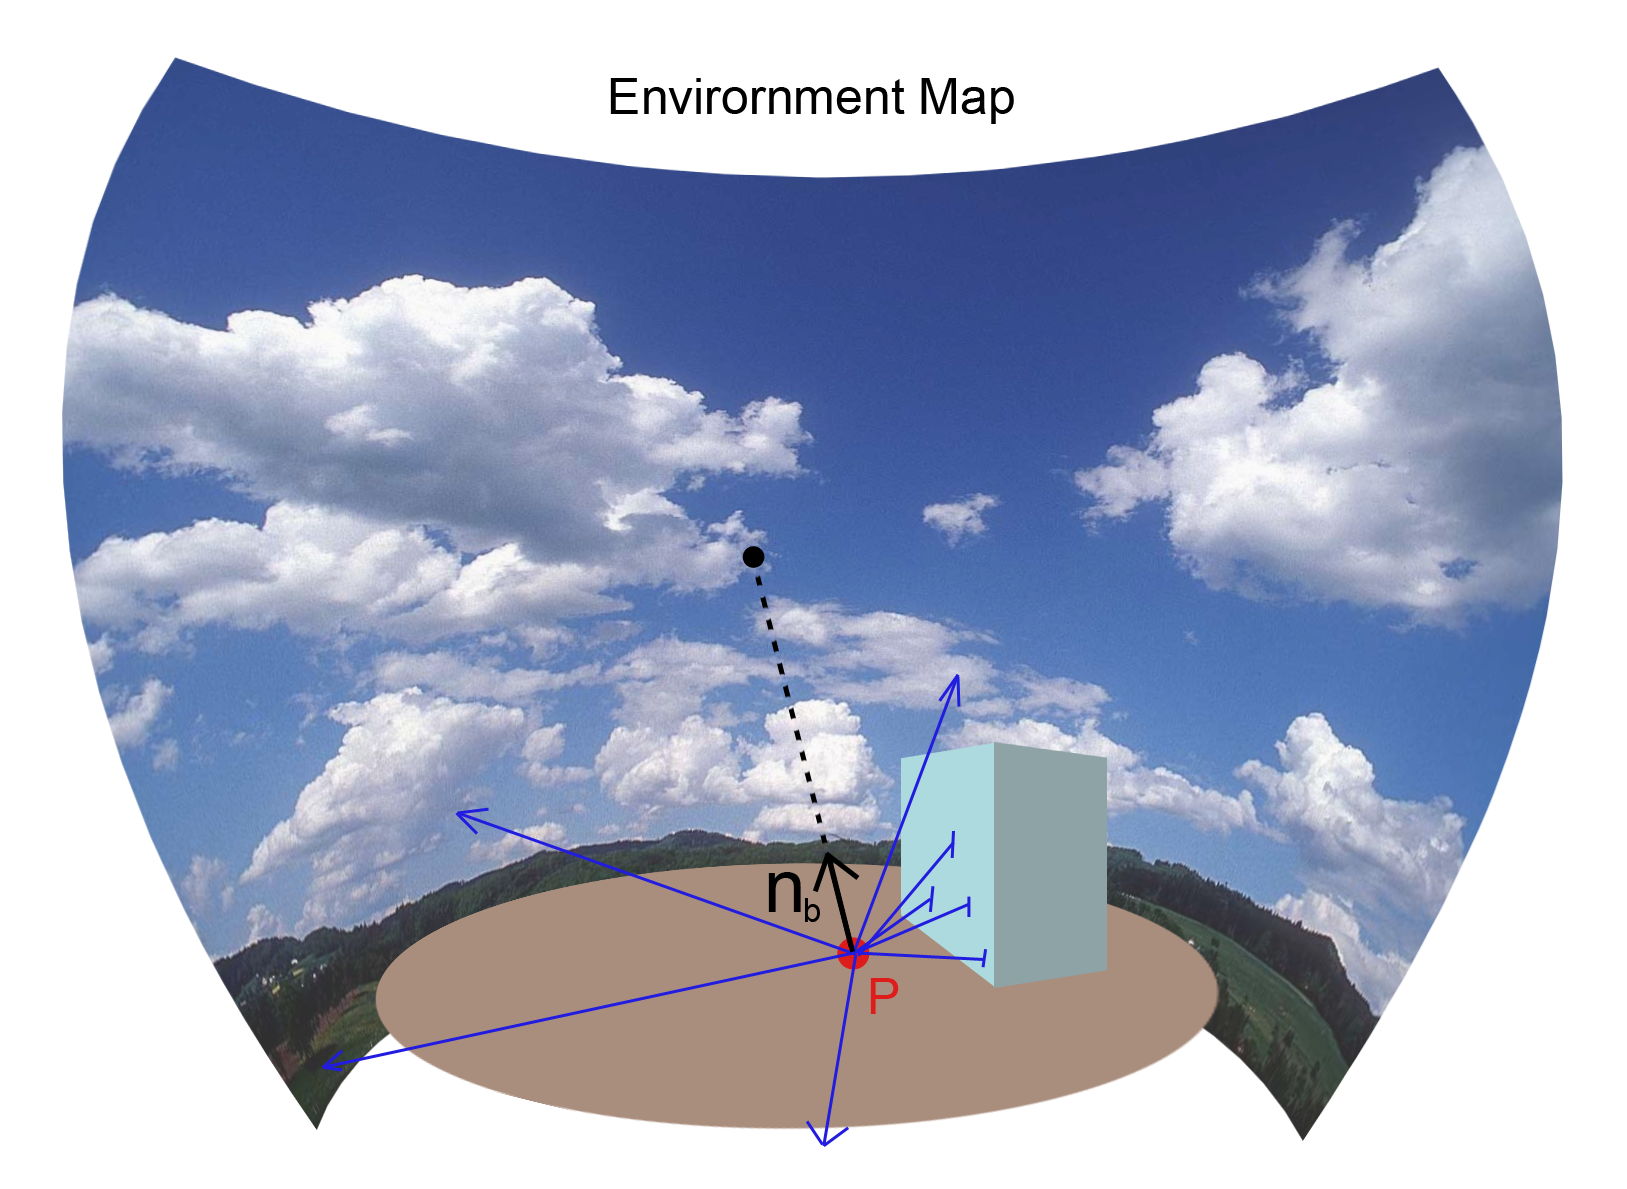
\includegraphics[width=0.6\textwidth]{Theory/overview}\caption{Overview of ambient occlusion.}\label{fig:overview}
\end{figure}
The accessibility at point P is determined by shooting rays out from the hemisphere surrounding the surface around P. The number of rays that does not hit other objects determines the accesibility. The average of the unoccluded rays is the bent normal that can be used to make a lookup into an envirornment map such as a light probe.
\section{Mathemathical Foundation}
Ambient Occlusion as all other realistic rendering methods tries to approximate the rendering equation:
\[ 
L_o(\textbf{x},\overrightarrow{w}) = 
L_e(\textbf{x},\overrightarrow{w}) +
\int_{2\pi}
 f_r(\textbf{x},\overrightarrow{w}',\overrightarrow{w} )L_i(\textbf{x},\overrightarrow{w}')\cos\theta dw'
\]
We will aproximate this with the Monte Carlo estimator\cite{Dutre2001}:
\[ 
L_o(\textbf{x},\overrightarrow{w}) = 
L_e(\textbf{x},\overrightarrow{w}) +
\frac{1}{N}
\sum_{i=1}^N \frac{ 
 f_r(\textbf{x},\overrightarrow{w}',\overrightarrow{w} )L_i(\textbf{x},\overrightarrow{w}')\cos\theta
}
{
pdf(\overrightarrow{w}_i')
}
\]
if we only consider diffuse reflectance then the BRDF is equal to the BRDF for Lambertian reflectance:
\[
 f_r(\textbf{x},\overrightarrow{w}',\overrightarrow{w}) = \frac{R_d}{\pi}
\]
Then the expression becomes:
\[ 
L_o(\textbf{x},\overrightarrow{w}) = 
L_e(\textbf{x},\overrightarrow{w}) +
\sum_{i=1}^N \frac{ 
\frac{R_d}{\pi}L_i(\textbf{x},\overrightarrow{w}')\cos\theta
}
{
pdf(\overrightarrow{w}_i')
}
\]
This expression can be evaluated directly by rejection sampling. However a better approach would be to simplify the expression even more. A good probability density function would therefore be\cite{Dutre2001}:
\[
pdf((\overrightarrow{w}_i')) = cos\theta / \pi
\]
The goal is therefore to find a sampling method that has this probability density function. One is\cite{Dutre2001}:
\[
\overrightarrow{w}_i' = (\theta,\phi) =
(\cos^{-1}\sqrt{r_1},2\pi r_2)
\]
Where r1 and r2 are random numbers between 0 and 1.
When this sampling method and a visibility function denoted V is used to describe incident illumination the equation finaly becomes:
\[ 
L_o(\textbf{x},\overrightarrow{w}) = 
\frac{1}{N}
\sum_{i=1}^N \frac{ 
\frac{R_d}{\pi})V(\textbf{x},\overrightarrow{w}')\cos\theta
}
{
cos\theta / \pi
}
\]
\[ 
L_o(\textbf{x},\overrightarrow{w}) = 
\frac{1}{N}
\sum_{i=1}^N
R_d V(\textbf{x},\overrightarrow{w}')
\]
\[ 
L_o(\textbf{x},\overrightarrow{w}) = 
\frac{R_d}{N} \sum_{i=1}^N V(\textbf{x},\overrightarrow{w}')
\]
Where V is equal to 1 if the direction is unoccluded and 0 otherwise. In a raytracer this is normally done by casting N rays with origin in the surface point being sampled with a cosine weighted random direction in the point's hemisphere, and divide the result by N. A similar approach is used to calculate the bent normal. This is the sampling method used in Landis' paper\cite{Landis2002} but other papers choose not to include the cosine term in the ambient occlusion integral to start with \cite{KRES2011}. Some also choose to let V return a value between 0 and 1 depending on the distance to the occluder where V returns 1 if the occluder being hit is farther away than a certain treshold \cite{McGuire:2010}. 
  
\section{Envirornment maps \& High Dynamic Range Imaging}
\label{sec:environment_maps}
As mentioned earlier the bent normal can be used to do a lookup into an image. Most often this image comes in the form of a light probe, which is an omnidirectional image that stores incident light at a certain point in space. Since the human visual perception is able to detect a high range of luminosity values, a high dynamic range format such as RGBE is often used. In RGBE the fourth byte stores an exponential value used to modify the RGB value. This allows the format to have the same range as floating point values. This way it can handle both very bright and dark pixels. The formula for converting RGBE value is simply:
\[
R_w = \frac{R_m + 0.5}{256} 2^{E-128} \]\[
G_w = \frac{G_m + 0.5}{256} 2^{E-128} \]\[
B_w = \frac{B_m + 0.5}{256} 2^{E-128} \]\[
\]
When the light probe is used to illuminate a diffuse surface the most used method is to sample the image in a region around the point sample from the bent normal. This way the lookup becoems blured which gives a more realistic look when used to color a diffuse surface\cite{Landis2002}.
\section{Lightprobe lookup}
A lightprobe is stored as a latitude longitude map as shown on figure \ref{fig:probe}.
\\ \\
\begin{figure}[h]
	\centering
	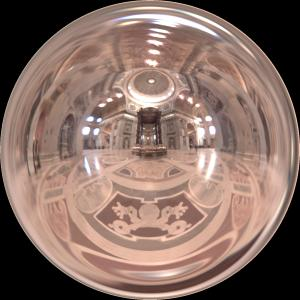
\includegraphics[width=0.4\textwidth]{Theory/example_probe}
\caption{Example of a light probe from St Peter's Basilica, Rome. Source\cite{website:PaulDebevec}}\label{fig:probe}
\end{figure}
\\ \\
When sampling a light probe it is therefore necessary to convert the 3 dimensional direction of the bent normal into a set of uv coordinates. We will now derive how. Since it is custom to have the center of the lightmap be the upwards direction we get that the base of the uv coordinates should be:
\[
(u,v) = (\frac{1}{2}, \frac{1}{2})
\]
the next part is to determine at what distance and in what direction from the center of the texture we should sample. Since we start from the middle of the texture the distance should go from 0 to 0.5. We can obtain this range by taking the arccos of the z value and divide by two pi:
\[
dist = \frac{arccos(D_z)}{2\pi}
\]
The x and y values tells us in what direction from the center we should go out to get to the right position. We therefore have to get the normalized xy vector:
\[
direction = \frac{1}{\sqrt{D_x^2 +D_y^2}} (D_x,D_y)
\]
At the end we can rearange to end up with the following:
\[
r = \frac{arcos(-D_z)}{2\pi\sqrt{D_x^2 + D_y^2}} 
\] \[
(u,v) = (\frac{1}{2}) + rD_x,\frac{1}{2}) + rD_y)
\]
Where D\textsubscript{x}, D\textsubscript{y} and D\textsubscript{z} is the lookup direction. Here it is assumed that the z-axis is upwards. One has also to take care of the event where Dx and Dy is close or equal to zero in which case the function should return (0.5 , 0.5). \newpage
\section{Disadvantages of Ambient Occlusion}
The main problem with Ambient Occlusion is from the fact that it reduces the problem of finding incident light, to using the calculated bent normal to do a texture lookup in an envirornment map. Since the bent normal is the average direction of incident light, it can in certain cases point in a direction that is actually occluded as illustrated by figure \ref{fig:bent_normal}.
\\
\begin{figure}[h!]
	\centering
	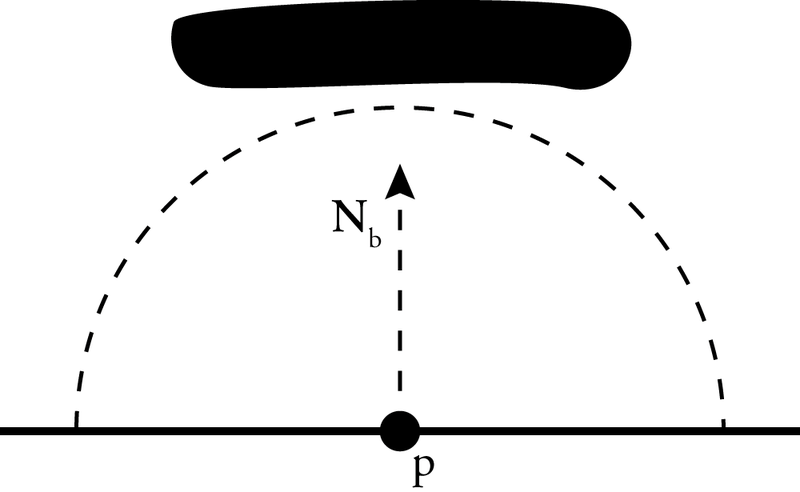
\includegraphics[width=0.5\textwidth]{Theory/bentNormalProblems}
\caption{The problem of using a bent normal Nb to find the irradiance at point P.}	\label{fig:bent_normal}
\end{figure}
\\ 
However since ambient occlusion is used to calculate the diffuse term the lookup into the envirornment map is usually blured which means this error is not so noticable.
\\ \\
The next section will cover our implementation of Ambient Occlusion.